\chapter{Fault Localization in Embedded Control System Software}\label{robot}

\section{Introduction}
Embedded systems are built and used everywhere in modern society. Controllers are the software part of some embedded systems
that control the behavior of the system. For example, consider a robot that has a high level goal of moving from one location to another. Therefore, bug-free control code is an important consideration. Our focus
is on algorithms that can help locate bugs in control code,
therebey reducing development time and improving the safety
of the system.  

Most low-level controllers, including the ones we evaluate, contain very few branch points. Generally, they are sequences of numerical computations that estimate the state of the system, compare to a reference state, solve an
optimal control problem and execute the solution. A bug in this context could be the result of an incorrect mathematical operation in the control code. This means that standard coverage
based fault localization techniques cannot in general be used because essentially the same sequence of statements is executed whether the output is faulty or not. Our prior work on value-based statistical fault localization attempted to develop techniques to locate faults  in numerical software. This is an extremely difficult problem. In this chapter, we focus on a subset of programs, namely embedded control systems. While embedded control systems are ubiquitous, the specific systems that we focus on in our work are robotic surgery systems. Using medical robot control systems, we develop an approach to automatically localize faulty statements in the control code.

The contribution of this chapter is: we implemented a java software with multi-threaded programming to send commands to the robotic surgery system and collect trajectory data; based on previous work, we developed a fault localization algorithm to localize the fault in embedded control system of medical surgery robot. In the following, we first provide additional background for our problem domain. Next, we describe our approach in detail, followed by empirical evaluation. Finally we give an overview of related work and conclude.

\section{Two Medical Surgery Robot Systems }\label{secrobot}
In this study, we use two prototype robotic surgery systems which are developed by CWRU Medical Robotics and Computer Integrated Surgery Lab \cite{MeRCIS}. The first robot is Small Animal Biopsy Robot(SABiR) \cite{bebek2008design}. The second robot is Beating Heart Robot(BHR) \cite{bebek2007whisker, bebek2006model}.

\subsection {SABiR}
SABiR is a five-degree-of-freedom (DOF) parallel robotic manipulator which is designed to take biopsies or deliver therapeutic drugs at targets in live small animal subjects. The robot has high position resolution and can realize dexterous alignment of  the needle before insertion. The desined accuracy of SABir is better than 250${\mu}m$. Figure \ref{sabir} shows an image of SABiR robot. 

The robot consists of a need mechanism held by two 5-bar linkage mechanisms, referred to as the front and rear stages. There are two DOF (up/down, left/right) in the front stage and three DOF (up/down, left/right, rotate forward/rotate backward) in the rear stage. The robot’s hardware state is characterized by its five joint angles. The robot’s needle position and direction can be transformed from 5 joint angles using a bijective inverse kinematic function.

\begin{figure*}[!thpb]
\centering
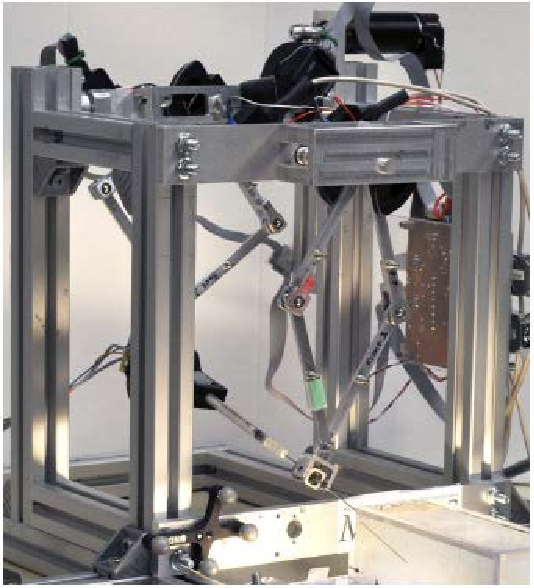
\includegraphics[width=0.6\textwidth]{chapter5_SABiR.pdf}
\caption{SABiR: The robotic system for image-guided needle-based interventions on small animals.}
\label{sabir}
\end{figure*}

\subsection{BHR}
BHR is a manipulator that will allow minimally invasive beating heart surgery\cite{bebek2008robotic}. It uses a three DOF robotic platform employing a PHANTom premium 1.5A haptic interface \cite{cavusoglu2001kinematics} as the robotic mechanism. The robot is composed of a base rotation an’sd a four-bar linkage, holding a tool arm. The DOF are driven by three motors: one actuating the base rotation, and two actuating the four-bar linkage in parallel. The joint angles are measured by quadrature encoders. The robot’s hardware state is characterized by its three joint angles, and there is a bijective inverse kinematic function to map any position and direction of robot’s end effector to a set of joint angles. Figure \ref{bhr} shows an image of BHR robot.

\begin{figure*}[!thpb]
\centering
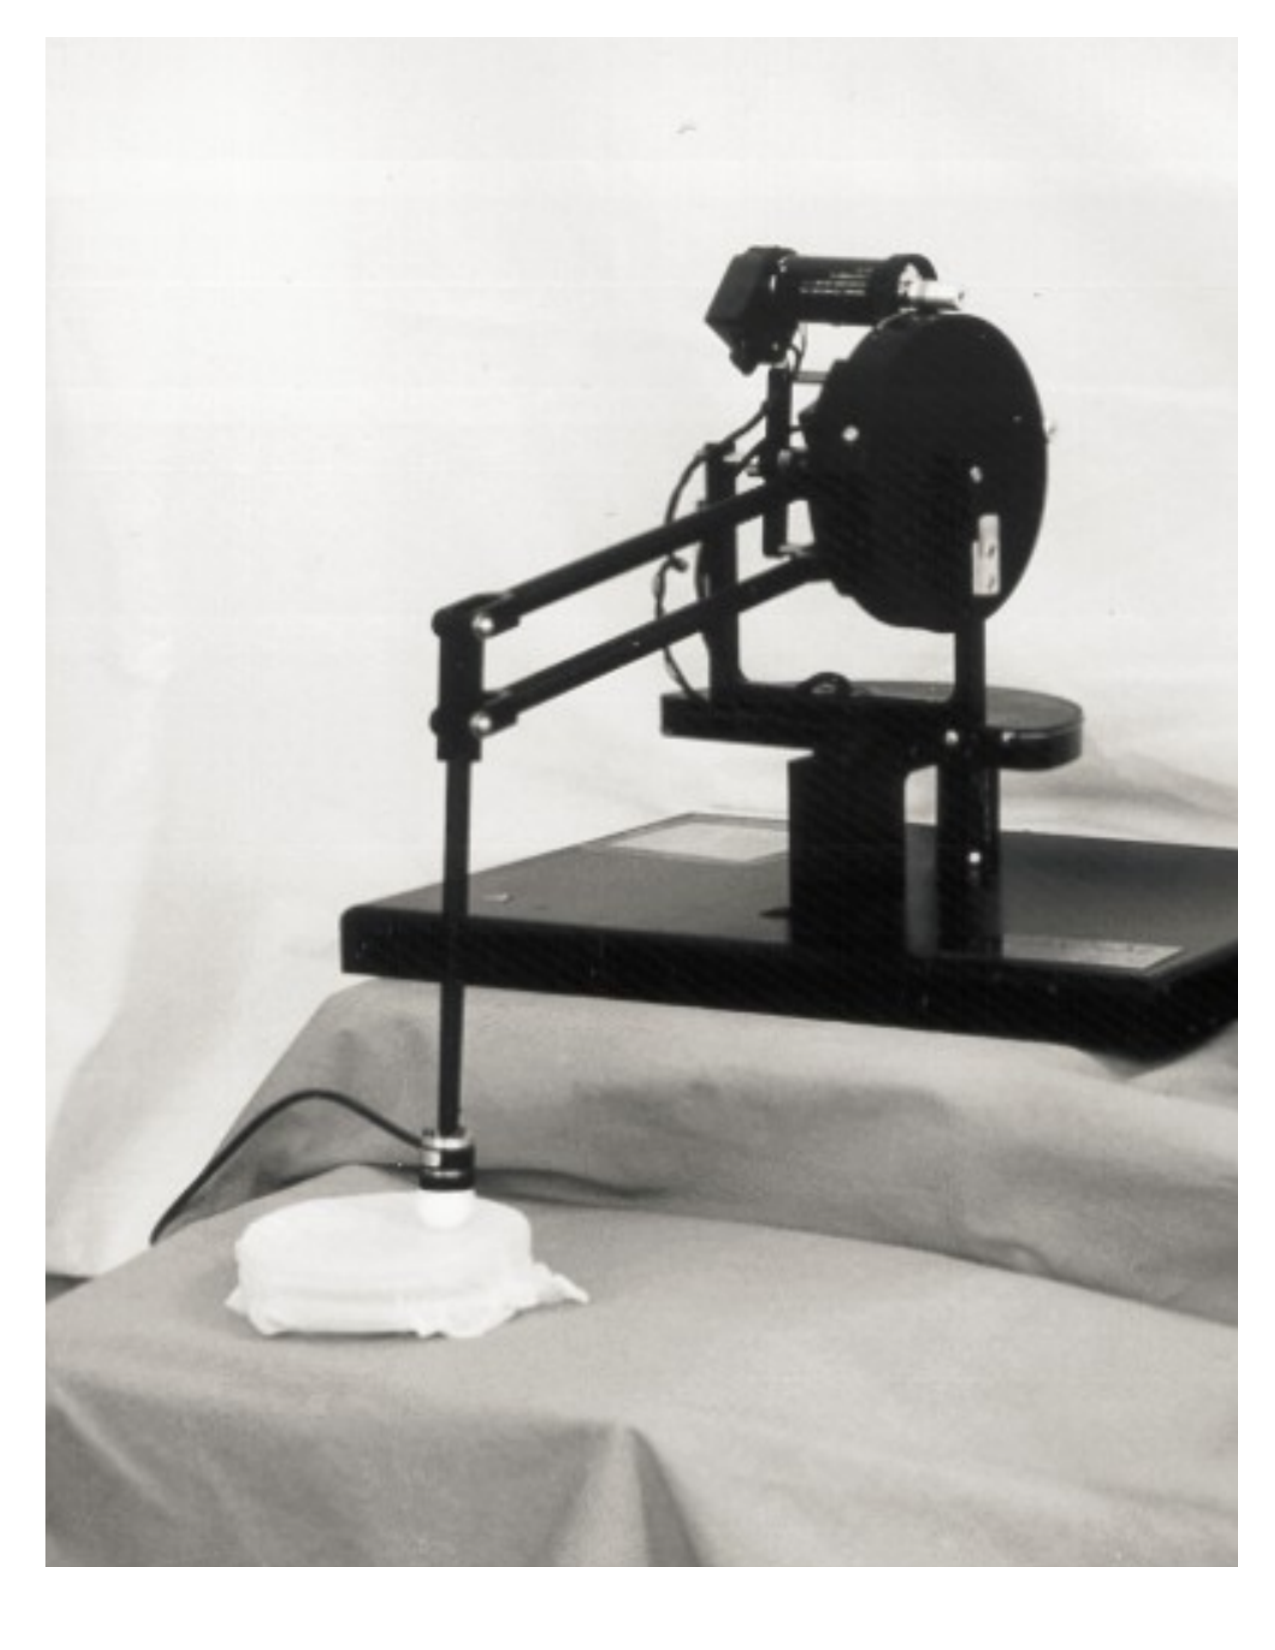
\includegraphics[width=0.6\textwidth]{chapter5_BHR.pdf}
\caption{BHR:Beating Heart Robot}
\label{bhr}
\end{figure*}

\section{Robot Simulation and Control}\label{robotsimulator}
The first part of our framework involves the development of an accurate simulator to ``stand in'' for the actual robot. 

For SABiR we have developed models for the kinematics and inverse kinematics for this robot~\cite{hwang2009kinematic} in prior work. We use these to create a simulation of the robot, implemented in Simulink, in which the robot’s motors are each represented as third-order transfer functions. The simulator is designed to be a modular component of the system, in the sense that it can be seamlessly swapped with the controller of the actual robot.

The environment simulation mainly contains two parts. The first part is two gel blocks to simulate the "tissue" in the workspace of the robot.  The second part is a needle force model to simulate the resisive force caused by the combined frictional, cutting, and stiffness forces produced when the needle is inside the gel block. The cutting force is caused by the needletip piercing the gel block and provides a resistance to the needle’s motion during insertion into the gel block.  The frictional force is produced by the friction between the needle body and the walls of the channel in the gel block, and resists the needle during insertion and extraction. The stiffness force is caused by the gel block’s tendency to resist sideways motion of the needle, i.e., any motion not in the direction the needle is pointing. In this way, realistic and distinguishable forces can be produced by any possible motion of the needle. The needle model is described in detail in~\cite{Russell2012}.

We use a simple low level controller to control the simulation. After calibration the robot’s initial location is called its ``home'' point. The controller can then be given new points and orientations to move the needle to. A ``reference'' trajectory is computed using linear interpolation. Velocities along this trajectory are set to be mainly constant, with fast acceleration and deceleration at the start and end (subject to a desired maximum acceleration). We then use a PD controller to follow this trajectory to guide the needle to the end point.

For BHR, we use models for the kinematics and inverse kinematics developed in our prior work \cite{bebek2007whisker} to create a simulation of the robot, implemented in MATLAB Simulink. In the simulations, the dynamics of each of the robot’s degrees of freedom are represented as sixth-order transfer functions. The environment of this robot consists of simulated heart and breathing motions, which the robot arm needs to follow. The BHR system uses a Receding Horizon Model Predictive Control based robotic motion control algorithm. As part of the motion control algorithm, the nonlinearities of the system (i.e., gravitational effects, joint frictions, and Coriolis and centrifugal forces) are also canceled. The controller has a sampling rate of 2 kHz.

\begin{figure*}[!thpb]
\centering
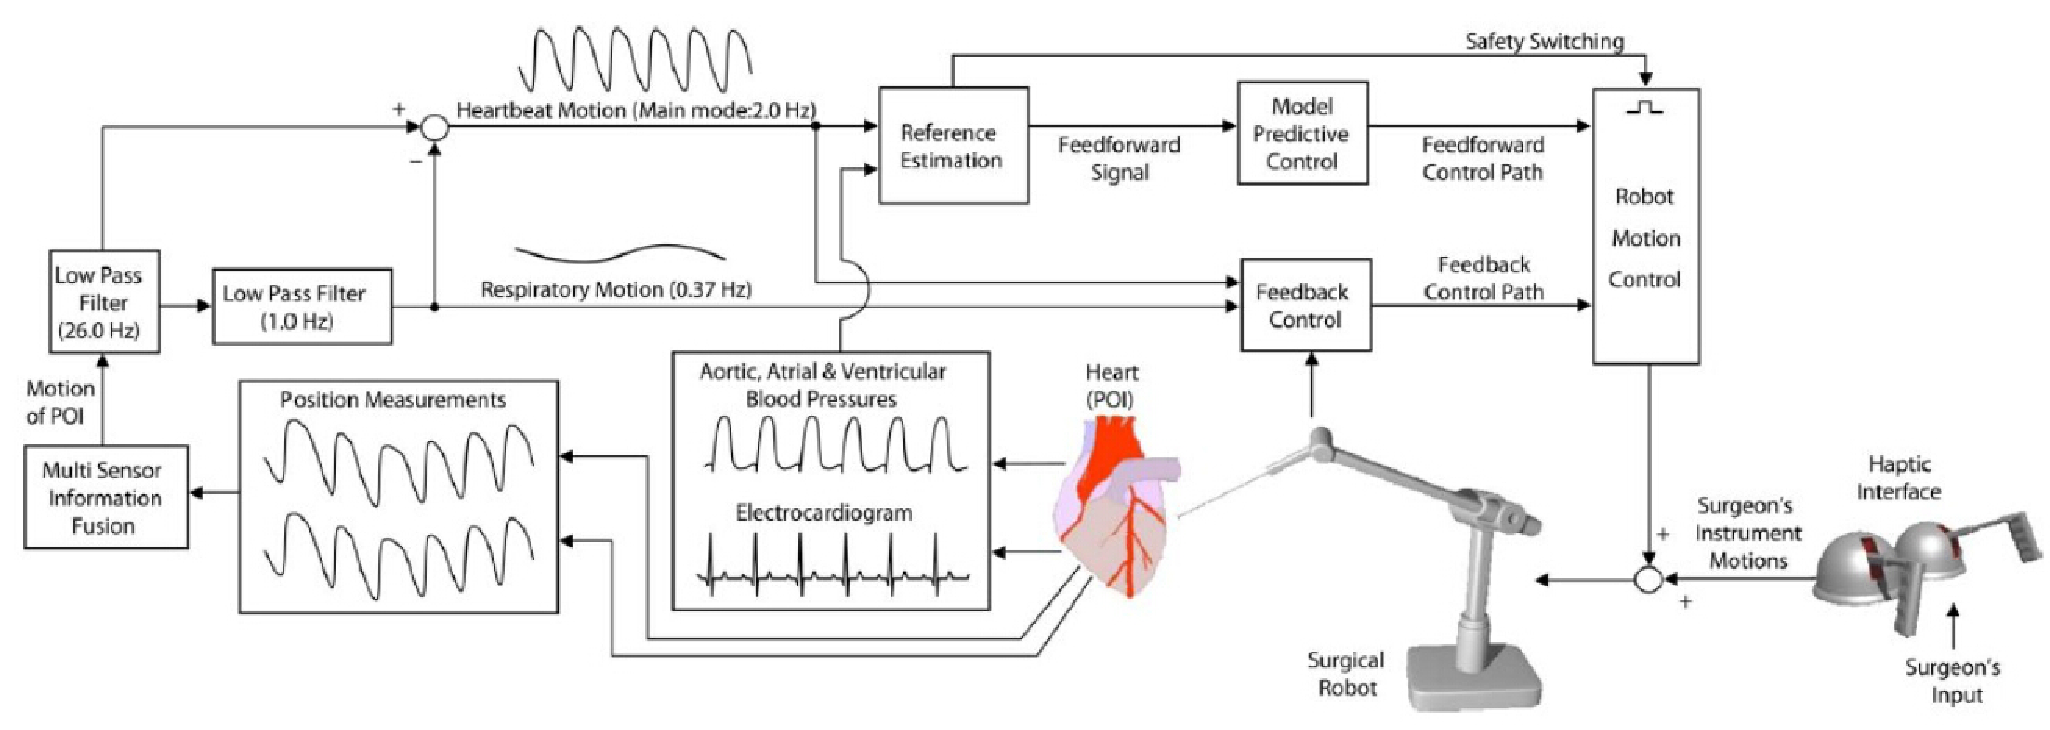
\includegraphics[width=\textwidth]{chapter5_BHR_control.pdf}
\caption{Control architecture for BHR}
\label{bhrcontrol}
\end{figure*}

The control architecture is shown in Figure \ref{bhrcontrol} \cite{bebek2007whisker, tuna2013heart}. . In the figure, sensors collect the blood pressure and electrocardiogram directly from the heart. Then they send the data to multi-sensor information fusion, which combines all the information and estimates the reference trajectory. Finally, the robot motion control block will drive the robot by following the reference estimation.

\section{Software Architecture and Data Collection}\label{softwareframe}

\subsection{Software Architecture}
For SABiR, we build a software system on top of the low-level controller. When a user interacts with the robot, this is what they see.  This system has three components: a GUI, a task delegator, and a robot proxy \cite{liangframework}. Figure~\ref{sabirsw} shows the information flow between these when the robot performs a high level insert/extract needle operation.

\begin{figure*}[!thpb]
\centering
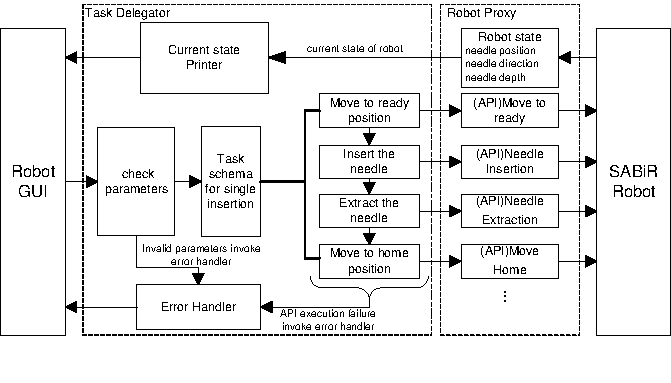
\includegraphics[width=\textwidth]{chapter5_SABiRsw.pdf}
\caption{Software Architecture of SABiR}
\label{sabirsw}
\end{figure*}

The software we build has a graphical user interface (GUI) that allows a user to view the current robot state and specify high level actions such as ``insert needle.'' For each such command, the GUI then lists all parameters whose values are needed to be input or adjusted. The data is then sent to a ``task delegator'' component. This first checks the validity of input parameters for the specified operation; for example, it ensures that target locations are within the robot’s workspace. It then decomposes a complex task into a set of basic needle motions that can be accomplished by calls to the API for the robot (or the simulator). The delegator is equipped with different schemas to decompose different high level tasks. It then invokes the robot API to handle these decomposed tasks. As the task is being executed, it updates the robot’s state on the GUI. If an error occurs, it is responsible for stopping the current action and alerting the user. The last stage, the ``robot proxy,'' handles communications with the robot (or simulation) and low-level operations and collects low-level sensor data from the robot (or simulation). This design ensures that when the simulation is replaced by the actual robot, only the last stage needs to be modified. Specifically, additional communication and synchronization code will be used to handle communications with the robot’s controller (built on XPC) and to ensure that data collection between the software and hardware is properly logged.

\emph{1)}	Robot GUI: The robot GUI provides a graphical user interface through which user can view the robot state and issue commands to control the behavior of the robot. When user send a command to robot, the GUI will list all the parameters required by the command for user to input or adjust their values.

\emph{2)}	Task Delegator: The task delegator is the bridge between the robot and GUI.  If the user initiates a complex task, it is decomposed in the task delegator into a set of basic actions that can be accomplished by robot API calls. Take Figure \ref{sabirsw} as an example, when a single insertion is issued from the GUI, the task delegator does the following:

\emph{a)}	Collects and checks parameters: To make sure the user provided appropriate information for the specified task, the task delegator collects the parameters provided by the user and checks their validity . For a single insertion, the task delegator mainly check whether the insertion will reach the position out of the workspace of the surgery robot.

\emph{b)}	Decomposes the task and invokes robot API to perform the task:  If the parameters are valid, the task delegator and then decomposes the task into a set of basic actions and invokes the robot API to control the robot in performing the task. For task decomposition, the task delegator provides different kinds of schemas to dealing with different types of tasks. For example, a single insertion will be decomposed into four basic actions: move to ready position, insert the needle, extract the needle and move back to home position. Each basic action has an corresponding function in API, which can control the robot to accomplish the action.

\emph{c)}	Displays task status via the GUI: While the task is processing, the task delegator displays its current status and any error reports to the user via the GUI. For a single insertion, the task delegator continuously update the following information on the GUI: needle position, needle direction, the current time of the operation and which basic action the robot is doing. If any error happens during the task processing, the task delegator will stop the task and inform user through the GUI.

\emph{3)}	Robot Proxy: The robot proxy provides the robot API, which is a set of basic operations for controlling the robot and for checking its status. There is one version of the proxy for the actual robot and another for the robot simulator. Also, the active robot proxy records the state of the robot (e.g., its current needle position and direction).The basic operations includes robot initialization, move, insertion, extraction, move back to home position, stop robot,  reset robot parameter and etc.There is one version of the proxy for the actual robot and another for the robot simulator. To perform a specified basic operation, two API functions is involved. First, a function will be called to generate the reference trajectory of the operation. The reference trajectory will be temporally stored in robot proxy. Next, a function named \emph{runRobot} will be called to send the reference trajectory to the robot. Then the robot will move its needle to perform the operation by following the reference trajectory. Because reference trajectory generation algorithm is identical under different platforms, when the Robot’s platform is changed (e.g., from simulator to actual robot), we only need to change the \emph{runRobot} function to fit the new platform.

For test purposes, the software system is used with the robot simulator. In the future, we will use it to control the actual robot. In our software framework, robot proxy is the only part to communicate with the robot(hardware). Thus, the robot GUI and task delegator will not change, but the robot proxy will be replaced by a new one which can talk to the actual robot. The robot proxy for actual robot provides the same API operations as the one for simulator. But the implementation of each robot API operation will change to fit the real robot platform. Specifically speaking, two robot proxy has different \emph{runRobot} functions.

\subsection{Data Collection}\label{subsec:datacollection}
We build the entire architecture to be easy to monitor and log. We base the data collection subsystem on the producer/consumer synchronization technique. We collect software execution data at the function level. That is, calling each function in the robot API
creates an object, which records the software state of the function’s execution. This object is sent to a buffer queue through the producer. When the hardware data is available, the consumer thread starts to get the corresponding software state object from the queue and records both software data and hardware data in a user readable format. For example, when the robot begins to insert the needle, two software state objects are created and sent to the buffer queue. The first records the software states like action name ``insert'', depth of the needle inside tissue during the reference trajectory generation. The second records variables such as Motor Speed Error, which are estimated by the software after hardware data is available. Then another object is created to record only the hardware data of the action ``insert'' and sent to the buffer queue. When the consumer is not writing, it continuously takes objects out of the buffer queue and puts them into a local queue. When the consumer gets an object with only hardware data, it starts writing. While it is recording the data, the system can continuously transmit additional software data through the Producer as long as the buffer queue is not full.

\section{Dynamic Bayesian Networks}\label{secdbn}
Based on the collected data, we use Dynamic Bayesian Networks(DBNs) \cite{liang2013detection} to model the time-evolution of the state space of the embedded control system. We use $S_t$ denotes a set of variables which characterized the state of control system at time $t$. DBNs are first order Markov model that represent the  probability of the next state given the current one, i.e $Pr(S_{t+1}|S_t)$. The factored stated transition distribution is defined by the equation:
\begin{equation}
\Pr ({S_{t + 1}}|{S_t}) = \Pr ({\pmb{V}_{t + 1}}|{\pmb{V}_t}) = \prod\limits_{i = 1}^n {\Pr (V_{t + 1}^i|{\pmb{V}_t})}  = \prod\limits_{i = 1}^n {\Pr (V_{t + 1}^i|\pmb{V}_t^{par(i)})} 
\end{equation}
where ${\pmb{V}_t} = \{ V_t^i\} $ denotes all the variables at time $t$. ${\pmb{V}_t^{par(i)}}$ denotes all the variables at time $t$ that have an effect to ${V_{t + 1}^i}$. Figure \ref{dbns} shows an example of DBN. Each node in the figure is associated with a conditional probability distribution (CPD), denoted as $\prod\limits_{i = 1}^n {\Pr (V_{t + 1}^i|\pmb{V}_t^{par(i)})} $, which is the probability distribution of $V^i$ given all the nodes in the previous time step that have an edge to it. From the equation above, the probability of the current state given the previous state equals the product of the CPD of each variable in the current state.
\begin{figure*}[!thpb]
\centering
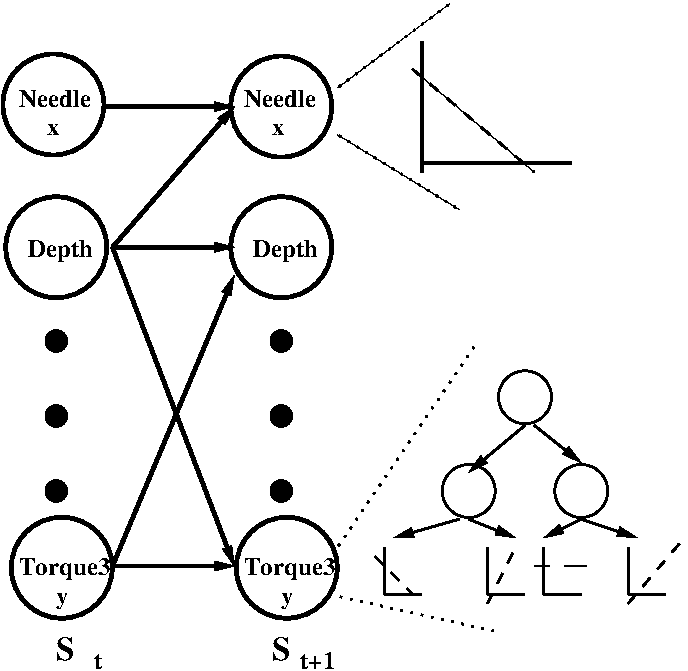
\includegraphics[width=0.6\textwidth]{chapter5_DBN}
\caption{Example Dynamic Bayesian Network}
\label{dbns}
\end{figure*}

To model CPDS, we applied two different models:{\it linear Gaussian model} and {\it regression tree model}. Because the robot controllers are designed to maintain a constant velocity in each high level action, we use {\it linear Gaussian model} to model some state variables which vary at a linear time rate from time $t$ to time $t+1$. For example, the variable represent $x$ axis of the needle tip position is one of those variable. For variables which have nonlinear variation from $t$ to $t+1$, we use a regression tree model for the CPB. In chapter 4, we have discussed the structure of regression tree model and mentioned that regression tree can model the nonlinear relationship between the predictors (input variables) and the response (target variables). In this work, we trained a DBN for each instrumented variable with the data from normal behavior of the robot control systems. The trained DBN will be used in identifying anomalous variables from the data of abnormal behavior of the robot control systems. For the detail of fitting the regression tree, please refer to our previous work \cite{cao2012classification}. In prior work, we have shown that this model and the training procedure yields very accurate models of normal hardware/software dynamics for the SABiR system. 

\section{Fault Localization Method}\label{dbnflalg}
In this chapter, the fault localization method is based on our previous work called FLECS, which is proposed by Liang and Ray at 2014 \cite{liang2015fault}. FLECS is a fault localization method in embedded control software with Dynamic Bayesian Networks. It contains two steps: (1) identifying anomalous variables and (2) identifying faulty statements. In this research, we modified the algorithm of identifying faulty statements in FLECS. The modified method is named as FLECS 2.0. 

\subsection{Identifying anomalous variables}
In section \ref{secdbn}, we mentioned that the DBNs are trained with the data collected from normal behavior of the robot. Thus, given a set of input variables ${\pmb{V}_t}$ which represents abnormal behavior of the system at time $t$, the output of DBN $ {\pmb{{\hat V}}_{i + 1}} $ will be the predicted normal behavior of the system at time $t+1$ based on the input ${\pmb{V}_t} $. If the values of some variables in the predicted state $ {\pmb{{\hat V}}_{i + 1}} $ are significantly different from the corresponding values of variables in the observed state  $ {\pmb{V}_{i + 1}} $, we identified these variables as anomalous variables. The identification of anomalous variables contains three steps.

First, we need to label the data of anomalous trajectories. An anomalous trajectory contains more than 10 thousand data points and each data point represents the state of the robot at a specific time $t$. But not all the data points in anomalous trajectories are considered as {\it "failing"} runs, because the bugs in the control software may only influence part of the trajectory. Thus, it is important to {\it extract} the {\it "failing"} runs from the data of the whole trajectories as the input of DBNs. This step can be done automatically by checking if the observed end effector position at time $t$ is same as the reference end effector position at time $t$. But since the data of observed end effector position comes from the hardware sensors, there is always some error between observed position and referenced position due to the noise of hardware.  In experiment, we label a data point as {\it "failure"} when the difference between of observed end effector position and reference end effector position exceeds a pre-defined tolerance $\epsilon$. This is similar to labeling the {\it "failing"} runs of numerical software. We need to point out that if programs producing complex outputs, manual inspection may be required to label the data.

Second, when the observation of a variable is different from the prediction of DBN. we need to set a threshold to decide if this is an anomalous variable. To address this problem, we maintain a range of normal likelihoods of $\Pr ({\pmb{V}_{t + 1}}|{\pmb{V}_t})$, which we calculate from the training data that was used to train DBNs.  Given the training data, which are all normal data points, we go through each pair of points and calculate the negative log likelihood (NLL) for all the variables. The negative log likelihood for a state $S_{t+1}$ given its previous state ${S_t}$ is computed as follows:

\begin{equation}
NLL({S_{s + 1}}|{S_t}) = \sum\limits_{i \in \{ Pred\} } {\frac{{{{(v_i^{pred}(t + 1) - {v_i}(t + 1))}^2}}}{{Var(i)}}} 
\end{equation}

where $Pred$ is the set of indices of predictable variables in the DBN, $v_{i}^{pred}(t+1)$ is the predicted value for variable $i$ at time $t + 1$, $v_{i}^{(t + 1)}$ is the real observed value for variable i at time $t+ 1$. $Var(i)$ is the variance of the CPD (in our case either regression tree model or linear Gaussian model) over training data. Then we pick the highest NLL among all the normal data points as the threshold. 

Third, for all the variables in the data with {\it "fail"} label, we use DBNs to predict of the variable values at the next time step. The we calculate NLL for each variable. Whenever the variable’s NLL is larger than the threshold, we consider it to be an anomalous variable. Using this approach, we can pick a set of anomalous variables.

\subsection{Identifying faulty statements}
After we get a set of anomalous variables which are identified by the algorithm above, what we need next is to translate those variables into controller code to locate the faults. To do this,
we choose the controller’s dynamic PDG, which was induced by traversing the PDG from $S{t-1}$, a normal input, to $S_t$ , an anomalous output. In our prior work FLECS, given a statement $s$, we sum the distances from the all statements containing the variables in the anomalous variable set as a total distance. The total distance is considered as the suspiciousness score of statement $s$. We rank the suspiciousness score and return a ranked list. But in this work, we proposed FLECS2.0, which modified method of calculating suspiciousness score of FLECS. 

\renewcommand{\algorithmicrequire}{\textbf{Input:}}
\renewcommand{\algorithmicensure}{\textbf{Output:}}
\begin{algorithm}
  \captionof{figure}{ {\it NUMFL} Algorithm}\label{flecs2.0}
  \begin{algorithmic}[1]
    \Require The software code of control system, simulator, trajectories with both normal and abnormal behavior
    \Ensure Ranked list of statements
    \State $D\leftarrow$ learned DBN from normal trajectories
    \State $T\leftarrow$ time index of start of anomalous event
    \State $t=T$; $BadVars\leftarrow \emptyset$; $WeightList\leftarrow \emptyset$; 
    \While  {$BadVars == \emptyset$ }
    	\State $BadVars\leftarrow$list of low-likelihoood variables at $t$ according to $D$
	\State $WeightList\leftarrow$list of weight of the variables in $BadVars$
	\State $t \leftarrow t+1$
    \EndWhile
    \State Sort $WeightList$ in descending order
    \State $P\leftarrow$ dynamic PDG of controller at $T$
    \State $O\leftarrow$ statements outputting $BadVars$ in $P$
    \State $Rank\leftarrow$ zero-element array of size number of nodes in $P$  
    \For  {$p$ a node in $P$ }
            \For  {$o$ a node in $O$ }
        		 \If{ p == o}
            		\State $Rank(p)=Rank(p)+30$
        		\ElsIf{$p$ is an ancestor of $o$}
			\State $d \leftarrow$ distance in $P$ from $p$ to $o$
			\State $r \leftarrow$ rank of the weight of $o$ in $WeightList$
            		\State $Rank(p)=Rank(p)+5/d+2/r$
        		\EndIf
   	    \EndFor
    \EndFor
    \Return statements in $P$ sorted by $Rank$
  \end{algorithmic}
\end{algorithm}


The algorithm of FLECS 2.0 is shown in Figure \ref{flecs2.0}. We first use DBN identified a set of anomalous variables $O$. Also, we assign a weight to each anomalous variable. The weight is equal to the difference between the NLL of the anomalous variable and the threshold. All the weights are stored in a list called weight list. Then given a statement $s$, we initialize its suspiciousness score as 0. We increase the suspiciousness score of $s$ in following two cases: (1) $s$ contains one or more variables in $O$. (2)$s$ contains a variable $p$ which is  the ancestor of a variable in $o \in O$ in PDG. The shorter the distance between $o$ and $p$ is, the more suspiciousness score $s$ received. The reason of increasing the suspiciousness score of $s$ in first case is straight forward. If $s$ is anomalous variable, we can infer that $s$ has erroneous state at $t+1$, which is possible to be the cause of the abnormal behavior of the system. For the second case, if $p$ is an ancestor of $o$, it means the value of $o$ is depend on the value of $p$ during the program execution. As a confounder, $p$ could be the cause of the abnormality of $o$ and thus $s$ should increase its suspiciousness score. 

We consider the first case is a stronger evidence that $s$ is faulty than the second case.  Assume the suspiciousness score of $s$ is increased by $m$ in the first case and is increased by $n$ in the second case, then we have $m>n$. The reason is that we have observed the abnormality of $s$ with the help of DBN in the first case. In the second case, the suspiciousness of $s$ comes from the fact that $p$ is a confounder of $o$,  but we did not observe the abnormality of $s$ from DBN.  Besides the above two cases, we also consider the weight of anomalous variables as a factor in suspiciousness score. If $p$ is an ancestor of $o$, we increase the suspiciousness score by a small value between 0 to $k$ according to the rank of the weight of $o$ in the weight list. The suspiciousness score increase more if the weight of $o$ has a higher rank in the list. In Figure \ref{flecs2.0}, we set $m=30$, $n=5$ and $k=2$. This is also the setting in our empirical evaluation.

Base on the algorithm in Figure \ref{flecs2.0}, we assigned a suspiciousness score to each statement in the control code. Then we sort all the suspiciousness scores in descending order. Once we get the sorted list, we can start debugging by tracing the statements all the way down from the top of the list. The debugging procedure is described as following steps: first we look at the first statement on the list. Then we localize it in the controller code and check if it is the bug that causes the anomalous event. If it is the buggy statement, we find the bug and fix it. If it is not the bug, we go to check the next statement in that list until we find the buggy statement.

\section{Empirical Evaluation}
We evaluate FLECS2.0 on the controllers of both SABiR and BHR. The controller of SABiR is written in MATLAB and has 330 lines of code in 6 functions, and contains 11 branches. We use the simulator we introduced in section \ref{secrobot} to generate both normal and abnormal trajectories of SABiR. The Normal trajectories are used to train DBNs and the abnormal trajectories are used to evaluate FLECS 2.0. The controller of BHR is also written in MATLAB and has 167 lines of code in 9 functions, and has no branches. We also trained DBNs for BHR with simulated trajectories. But for abnormal trajectories, we use the data collected from the hardware robot.

\subsection{Instrumenting the Controllers}
To collect data for our approach, we need to record the final values of variables after the controller finishes processing one time step. To keep the data collected reasonable, we chose to monitor 100 or fewer variables from each controller. We used two heuristics to determine which variables to monitor. First, for large matrices that are used in statements as a single entity (e.g. $X = A*B$), a candidate for monitoring is a single, randomly chosen element (from $X$ in this case). The rationale here is that if this statement is faulty, all the matrix elements are affected by it. However, if a statement uses a specific element from a matrix (e.g.$X(2, 2) = A(2, 3) * B(3, 2)$) then that element is a candidate for us to monitor. For matrices of size ten or less, however, every entry was a possible candidate for monitoring.

We use a second rule to prune the list of candidates determined above. Here, we select those variables that are "hub" variables in the controller’s PDG in that they influence many other variables' values. In our controllers, selecting variables that influence at least five other variables in the program gives us a reasonably sized set of variables to monitor. As a result of this selection process, we instrument 87 software variables from the controller of SABiR and 59 variables from the controller of BHR. The values of these variables are collected at every time step, after the controller finishes running, and used to generate training and testing data.

\subsection{Faulty Controllers}\label
To evaluate the techniques, we need buggy versions of the controllers. Through randomized testing we discovered one bug in the SABiR controller that triggers because of a missing check. This causes a subsequent square root computation to return a complex number of which only the real part is stored and processed, leading to anomalous behavior in the simulator. To generate additional bugs, we used mutation testing. Here we create a set of faulty versions of the controllers (mutants) through the randomized modification of elements of the code. This approach has been used in prior work \cite{liang2013detection}. We use four mutation operators: replace numerical constant, negate jump condition, change arithmetic operator, and add/subtract a small numeric value. We repeatedly randomly mutate an expression in the code and retain those which produce anomalous behavior. Through this process, we generated 10 faulty controllers for SABiR and 12 for BHR.

In the experiments, we use ESP-SCP and the original version of FLECS as baselines \cite{liang2015fault}.

\subsection{Methodology and Baselines}
We use 400 normal trajectories obtained through our simulator to train our DBN for SABiR and 10 trajectories to train a DBN for BHR. Each trajectory has 25,000 data points for SABiR and 11965 data points for BHR. For each trajectory generated with buggy versions of the SABiR controller that contained an anomalous event, we label the starting point manually by plotting the needle’s trajectory in MATLAB and comparing to the reference data. For BHR, we label points as anomalous using an automatic criterion, when the "end effector error" variable goes beyond a predetermined normal threshold.

Each technique we use returns a ranked list of statements in the controller code. We report the rank of the first faulty statement in this list. In the case of ties, we place the faulty statement in the middle of the set of statements with the same score, which simulates a developer having to consider half of this list before finding the fault. The results of our experiments are shown in Table \ref{flbhr} and Table \ref{flsabir}.

Table \ref{flbhr} shows the result of experiments on BHR. FLECS 2.0 performs better than ESP-SCP on 9 faulty controller versions, but performs worse than ESP-SCP on 3 faulty controller versions.  FLECS 2.0 performs better than FLECS on 8 faulty controller versions, but performs worse than FLECS on 2 faulty controller versions. There are also two faulty version that FLECS and FLECS 2.0 have the same performance. Bug 6 is particularly interesting, because we found that the automatic starting point labeling criterion did not work well, and the labeled starting point was around 10000 steps before the true starting point of the anomalous event. Without the correction procedure described in section \ref{dbnflalg}, the faulty statement is ranked 134 by FLECS 2.0. The rank improves to 25 after the correction, indicating that this procedure can help correct for errors in the automatic labeling process. Table \ref{flsabir} shows the result of experiments on SABiR. FLECS 2.0 performs better than ESP-SCP on 8 faulty controller versions, but performs worse than ESP-SCP on 2 faulty controller versions.  FLECS 2.0 performs better than FLECS on 5 faulty controller versions, but performs worse than FLECS on 4 faulty controller versions. There is one faulty version that FLECS and FLECS 2.0 have the same performance. The first bug for SABiR in Table \ref{flsabir} is a real bug.  An interesting aspect of this bug is that the variables that were being computed by the faulty statements were not selected for monitoring in our list of 87 (for SABiR) variables that constitute the software state in our DBNs. However, some data dependencies of that statement were selected, and since this statement was the only fault in this experiment, it "explained" many of these dependencies and so was ranked relatively highly. Overall, the experiment result shows that FLECS 2.0 outperforms ESP-SCP and original FLECS on two control system softwares. 

\begin{table*}[htbp!]
%\fontsize{10pt}{10pt}\selectfont
\centering
\caption{RANK OF THE FIRST FAULTY STATEMENT FOR BHR}
\label{flbhr}
      \begin{tabular}{|l|c|c|c|}
      \hline
Bug Index	&	ESP-SCP	&	FLECS	&	FLECS2.0	\\ \hline
1	&	85	&	73	&	15	\\ \hline
2	&	84	&	24	&	44	\\ \hline
3	&	60	&	97	&	18	\\ \hline
4	&	12	&	24	&	32	\\ \hline
5	&	13	&	14	&	9	\\ \hline
6	&	33	&	83	&	25	\\ \hline
7	&	81	&	61	&	12	\\ \hline
8	&	31	&	61	&	14	\\ \hline
9	&	11	&	14	&	56	\\ \hline
10	&	33	&	140	&	140  \\ \hline
11	&	81	&	90	&	22	\\ \hline
12	&	59	&	65	&	21	\\ \hline
\end{tabular}
\end{table*}

\begin{table*}[htbp!]
%\fontsize{10pt}{10pt}\selectfont
\centering
\caption{RANK OF THE FIRST FAULTY STATEMENT FOR SABiR}
\label{flsabir}
      \begin{tabular}{|l|c|c|c|}
      \hline
Bug Index	&	ESP-SCP	&	FLECS	&	FLECS2.0	\\ \hline
1	&	249	&	39	&	7	\\ \hline
2	&	1	&	3	&	26	\\ \hline
3	&	251	&	3	&	35	\\ \hline
4	&	42	&	2	&	36	\\ \hline
5	&	218	&	28	&	23	\\ \hline
6	&	10	&	27	&	21	\\ \hline
7	&	49	&	65	&	17	\\ \hline
8	&	6	&	23	&	5	\\ \hline
9	&	263	&	10	&	10	\\ \hline
10	&	39	&	3	&	13	\\ \hline
\end{tabular}
\end{table*}

\section{Related Work}
The work most closely related to ours involves using probabilistic models to identify bugs in programs. Liu et al. propose the SOBER method \cite{liu2006statistical}, which builds a probabilistic model for program predicates. If the probability that a predicate P evaluates to true in passing runs is significantly different from the probability that P evaluates to true in failing runs, P is judged to be related to program failure. SOBER models control dependences but not data dependences. 

Some papers have focused on software testing for MATLAB/Simulink applications. Zhan et al \cite{zhan2008search} proposed a search based framework to generate test data for a Simulink model. He et al \cite{he2011test} use an improved mutation testing technique to reduce the cost of test data generation for Embedded Simulink. This work does not address the problem of fault localization, however.

Most related research on the safety of medical robotic systems in the literature primarily focus on design of intrinsically safe systems, e.g. \cite{taylor2008medical,taylor1996computer,dombre2001intrinsically,duchemin2004medically}. A related approach in hybrid systems is parameter synthesis \cite{donze2009parameter}. Here system parameters, such as joint limits, power levels, mass, etc. are designed in such a way as to produce good behavior and minimize or eliminate risk and/or the system is designed to fail in a safe manner and come to a controlled halt so that it can be removed and the procedure completed manually. This is typically achieved by using actuators with limited power and speed, current limiters, etc. These approaches do not consider the software development process, however, and do not attempt to address the problem of developing tools to aid the development of the controller.

Online fault detection and diagnosis is a very well studied problem in general robotics and other hybrid systems (e.g.\cite{halder2007robust,mcintyre2005fault,verma2004real}). A common approach is to use probabilistic sequence models to represent the system and to perform online inference to detect when the system is in a faulty state. These models also typically focus on modeling the hardware and devote attention to efficient inference algorithms to account for the online setting. Recent work on diagnosis has started to look at software as well \cite{mikaelian2005model}, though at a coarse level.

\section{Conclusions}
In this chapter, we have presented and evaluated an algorithm to locate faulty statements in control software, which is widely used in many embedded systems including robots and vehicles. The characteristics of such low-level control systems make coverage-based fault localization techniques unsuitable. However, given the safety critical nature of many such systems, it seems valuable to design automated aids to developing them. Our approach assists in debugging such software by modeling the values of variables in the system. Given an anomalous event, it uses the model to find anomalous variables, which are then traced through the PDG to determine possible causes (statements). Experiments using two medical robot prototypes developed in our labs indicate the approach is promising.